\documentclass[11pt,letterpaper]{article}
\usepackage[lmargin=1in,rmargin=1in,bmargin=1in,tmargin=1in]{geometry}
\usepackage{style/quiz}
\usepackage{style/commands}

% -------------------
% Content
% -------------------
\begin{document}
\thispagestyle{title}


% Quiz 1
\quizsol The following relation represents a function:
	\[
	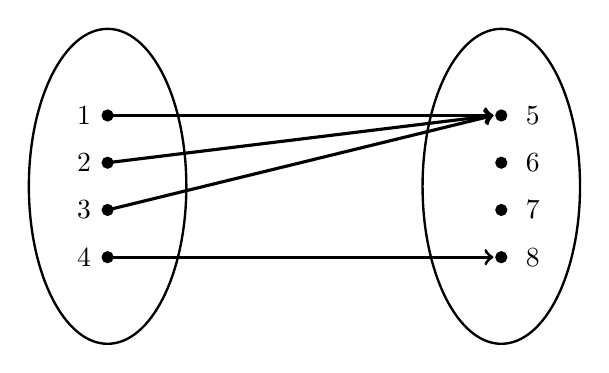
\begin{tikzpicture}
	% Ellipses
	\draw[line width=0.03cm] (0,0) circle (1 and 2);
	\draw[line width=0.03cm] (5,0) circle (1 and 2);
	
	% Nodes
	\draw[fill=black] (0,0.9) circle (0.07);
	\draw[fill=black] (0,0.3) circle (0.07);
	\draw[fill=black] (0,-0.3) circle (0.07);
	\draw[fill=black] (0,-0.9) circle (0.07);
	
	\draw[fill=black] (5,0.9) circle (0.07);
	\draw[fill=black] (5,0.3) circle (0.07);
	\draw[fill=black] (5,-0.3) circle (0.07);
	\draw[fill=black] (5,-0.9) circle (0.07);
	
	% Arrow
	\draw[line width=0.04cm,->] (0,0.9) -- (4.9,0.9);
	\draw[line width=0.04cm,->] (0,0.3) -- (4.9,0.9);
	\draw[line width=0.04cm,->] (0,-0.3) -- (4.9,0.9);
	\draw[line width=0.04cm,->] (0,-0.9) -- (4.9,-0.9);
	
	% Labels
	\node at (-0.3,0.9) {$1$};
	\node at (-0.3,0.3) {$2$};
	\node at (-0.3,-0.3) {$3$};
	\node at (-0.3,-0.9) {$4$};
	
	\node at (5.4,0.9) {$5$};
	\node at (5.4,0.3) {$6$};
	\node at (5.4,-0.3) {$7$};
	\node at (5.4,-0.9) {$8$};
	\end{tikzpicture}
	\]

\sol The statement is \textit{true}. A relation is a function if for every input, i.e. every value in the domain, there is one output. For each of the values 1, 2, 3, 4, we know the value of the output. It does not matter that several of the values get `sent' to the same value---only that we know what value they go to. \pspace



% Quiz 2
\quizsol If $C(x)$ is a cost function, then the $y$-intercept of $C(x)$ is the fixed costs. \pspace

\sol The statement is \textit{true}. The $y$-intercept of a function is the value where $x= 0$ (which means the function is intersecting the $y$-axis). But then we are looking at the value of $C(0)$, which represents the costs of producing zero items. But any costs associated with producing zero items must be a `baseline' cost for production, i.e. the fixed costs. 






























\end{document}